\documentclass[12pt]{article}
\usepackage{caption}
\usepackage{graphicx}
\usepackage{hyperref}
\usepackage[german]{babel}
\usepackage{amsmath}
\hypersetup{%
    pdfborder = {0 0 0}
}
\hypersetup{
    colorlinks,
    citecolor=blue,
    filecolor=blue,
    linkcolor=blue,
    urlcolor=blue
}
\renewcommand{\familydefault}{\sfdefault}
\renewcommand{\captionfont}{\small}

\author{Bernd Porr}
\title{Q-Lernen und ``Tiefes'' Q-Lernen}

\begin{document}

\maketitle
\section{Traditionelles Q-Lernen}

Q-lernen ist ein Lernalgorithmus wo eine Agentin selbständig
lernt ihre Belohnung zu maximieren.

\begin{figure}[!hbt]
\begin{center}
\mbox{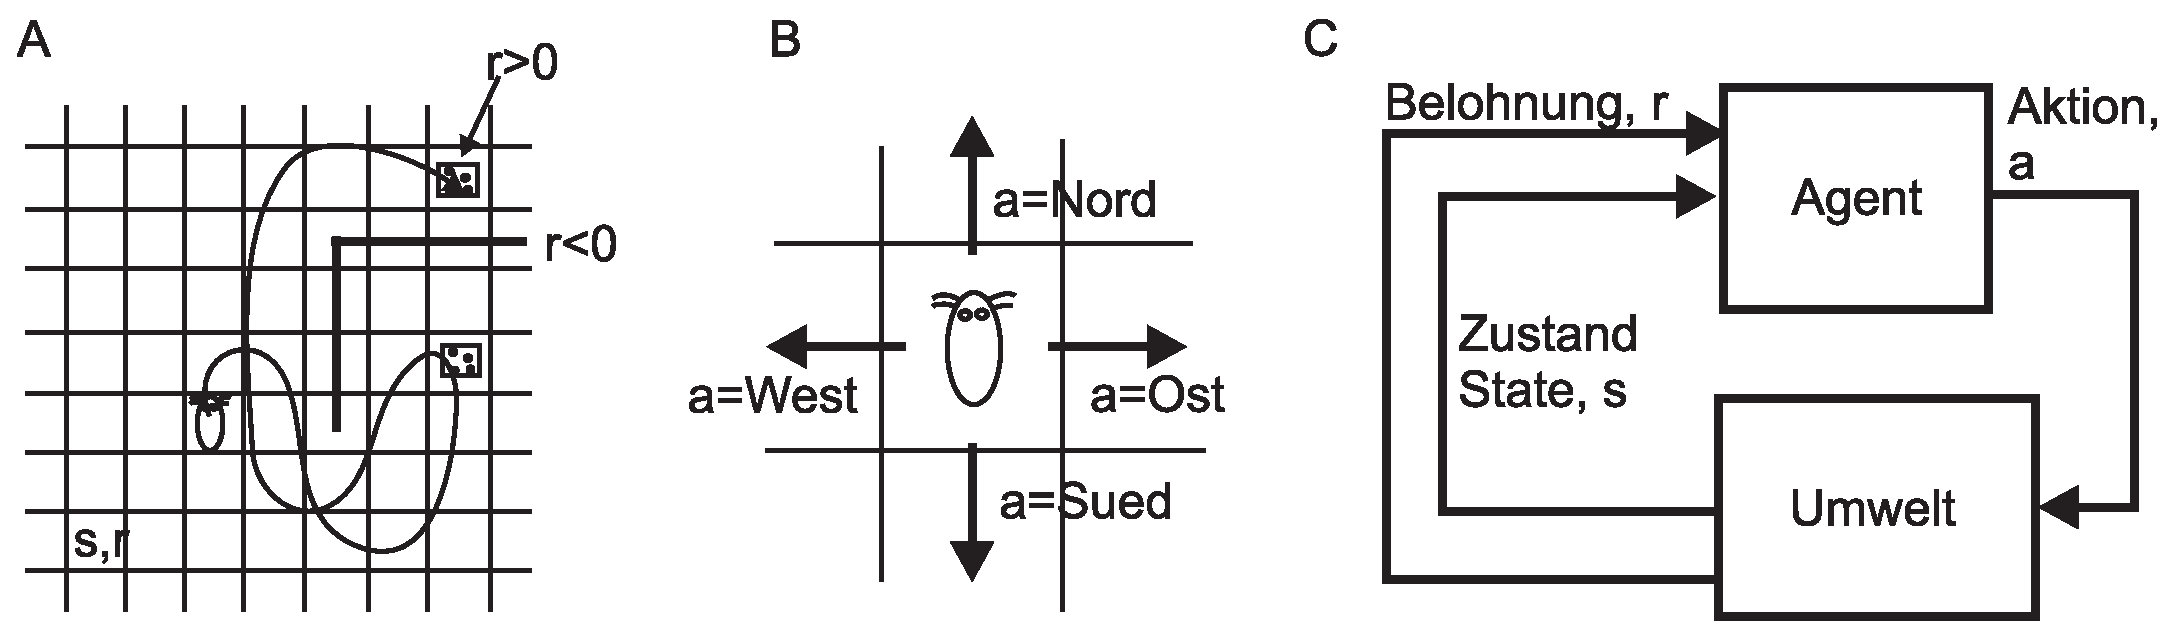
\includegraphics[width=\textwidth]{state_action}}
\end{center}
\caption{Zustandsraum und Aktionen einer autonomen Agentin (z.B eine Maus),
  die Futter sucht.
\label{state_action}}
\end{figure}

Abb.~\ref{state_action} zeigt eine klassische 2D-Welt, in der sich
eine solche Agentin (hier eine Maus) bewegt. Abb.~\ref{state_action}A
zeigt den Zustandsraum. In diesem Beispiel ist der Zustandsraum 2D, in
dem sich die Agentin bewegen kann. Manche Zustände sind durch Wände
verboten und bei anderen gibt es eine Belohnung (als ``Käse''
gekennzeichnet). Zustände werden mit $s$ gekennzeichnet und wenn sie
zum Zeitpunkt $t$ passieren, dann wird das als $s_t$
gekennzeichnet. Jeder Zustand besitzt auch eine skalare
Belohnungsvariable $r$, die positiv $r>0$ ist, wenn es eine Belohnung gibt
und negativ $r<0$, wenn der Zustand bestraft werden soll. Für alle anderen
Zustände ist $r=0$.

Abb.~\ref{state_action}B zeigt die möglichen Aktionen $a$, die die
Agentin durchführen kann. Eine Aktion bewirkt eine Bewegung von einem
Zustand $s_t$ zum Zeitpunkt $t$ zum Zustand $s_{t+1}$ und evtl gibt
es eine Belohnung ($r>0$) oder eine Bestrafung ($r<0$).

Abb.~\ref{state_action}C illustriert, wie man die Interaktion zwischen
der autonomen Agentin und Umwelt als geschlossenes System interpretieren. Jede
Aktion $a$ der Agentin erzeugt einen neuen Zustand $s$ und
gegebenenfalls auch eine Belohnung $r$.

\begin{figure}[!hbt]
\begin{center}
\mbox{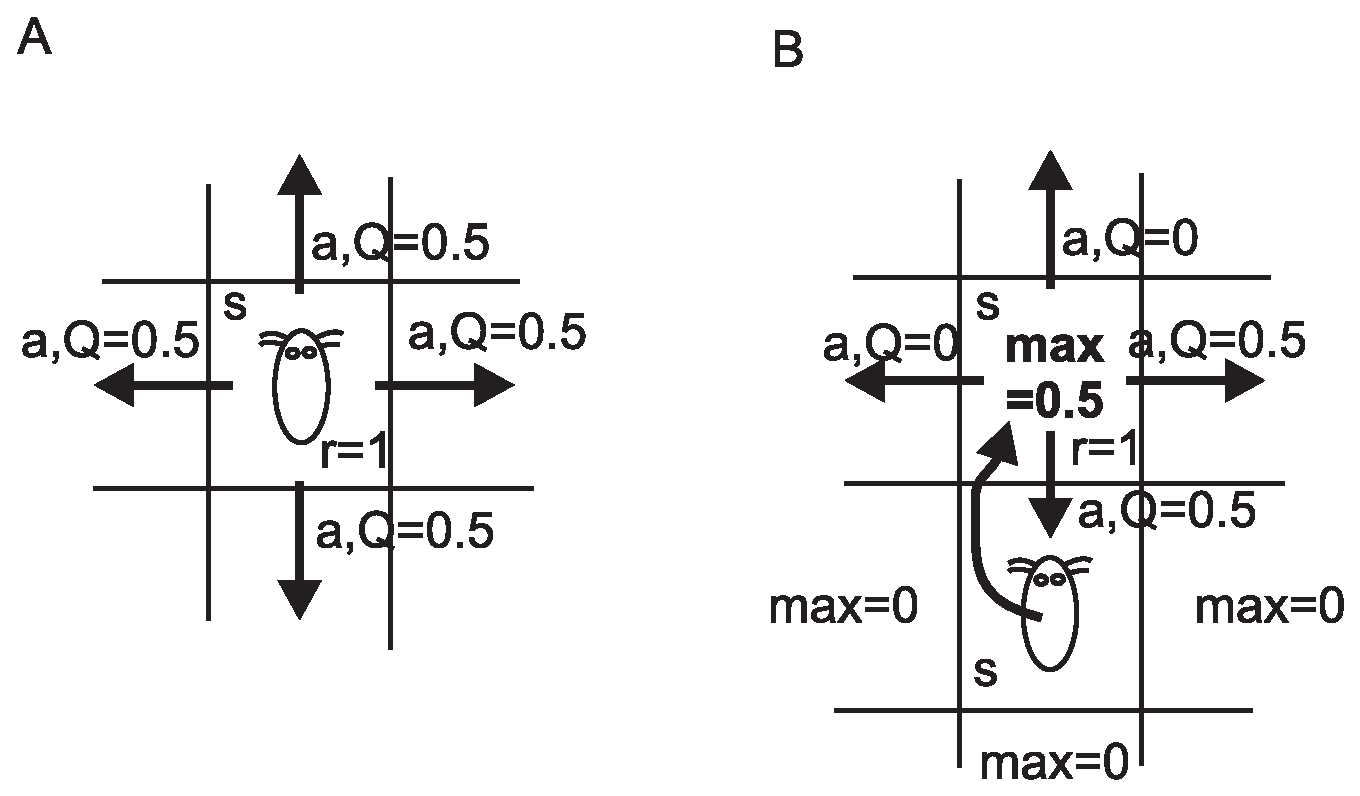
\includegraphics[width=0.75\textwidth]{learning_steps}}
\end{center}
\caption{Lernschritte von Q-learning. A) Die Agentin befindet
  sich direkt auf der Belohnung. Das führt dazu, dass alle
  Q-Werte gleichermaßen erhöht werden, z.B. auf $0.5$ mit
  einer Lernrate von $\alpha = 0.5$.
\label{learning_steps}}
\end{figure}

Die Frage stellt sich nun, wie die Agentin von jeder beliebigen Stelle
$s$ die Belohnungen findet. Das wird erreicht, indem jede Aktion $a$
bezüglich eines Zustandes $s$ eine Hilfsvariable erhält, die wir
$Q(s,a)$ nennen (siehe Abb.~\ref{learning_steps}A). Jede Aktion $a$ in einem
Zustand $s$ erhält damit verschiedene Q-Werte. Das Ziel ist es, den Aktionen
einen hohen Q-Wert zu geben, die maximale Belohnung versprechen. In diesem
Beispiel erhält jeder Zustand $s$ vier Q-Werte (Nord, West, Ost
und Süd). Anfänglich sind alle Q-Werte null werden dann mit Hilfe der iterativen Bellmangleichung bestimmt:
\begin{equation}
  Q(s,a) \leftarrow Q(s,a) + \alpha \underbrace{\left[ r(s) + \gamma \max_{a^\prime} Q(s^\prime,a^\prime) - Q(s,a) \right]}_{\delta(s,a)}
  \label{bellit}
\end{equation}
wo $\alpha$ die Lernrate ist und $0 < \gamma < 1$ der ``discount
Factor'' der zukünftige Belohnungen abwertet. Für die Beispiele hier
nehmen wir einfach an, dass $\alpha = 0.5$ und $\gamma = 1$ ist.

Die Q-Werte werden nun iterativ gelernt, wobei die Agentin
Zufallsaktionen $a$ durchführt und dann $Q(s,a)$ aktualisiert
wird. Die Agentin kann immer einen Schritt voraussehen, also quasi
über die Schwelle zu einem anderen Zustand gucken. Das wird in Q-Lernen
``Beobachtung genannt''. Mehr kann die Agentin nicht sehen. Am Anfang
sind all Q-Werte null. Nur die direkte Belohnung kann diesen Q-Wert von Null
erhöhen, was in Abb.~\ref{learning_steps}A gezeigt wird. Bei einer
Lernrate von $\alpha = 0.5$ ergibt das dann für alle Aktionen einen
Q-Wert von $0.5$.

Der entscheidende Trick ist aber nun, wenn bei der nächsten
Zufallswanderung die simulierte Maus einen Schritt vor der primären
Belohnung steht und $Q(s,a)$ nicht mehr überall null
ist. Abb.~\ref{learning_steps}B zeigt nun die Agentin einen Schritt
vor der Belohnung. Die Maus schaut also nun in die verschiedenen
Felder um sich herum und bestimmt dort den maximalen Q-Wert
$\max_{a^\prime} Q(s^\prime,a^\prime)$, vergleicht den mit dem
aktuellen Q-Wert $Q(s,a)$ und korrigiert dann den aktuellen Q-Wert
anhand der Lernrate. Aus diesem Grunde wird der Term $\delta(s,a)$
auch Vorhersagefehler oder im Englischen ``Reward Prediction Error''
(RPE) genannt.

Das Experiment in Abb.~\ref{learning_steps} wird nun mit der
Formel.~\ref{bellit} viele Male mit Zufallswanderungen bei einer
maximalen Laufzeit $T$ wiederholt, bis der Fehler $\delta$ im Mittel
Null ist also die Q-Werte sich nicht mehr ändern. Das Endergebnis gibt
dann eine Vorhersage der gesamten Belohnung in Abhängigkeit von $s$
und $a$:
\begin{equation}
  Q(s,a) = \sum_{t=0}^T \gamma^t r_t
\end{equation}
wo $T$ die Gesamtzeit ist, die Aufgabe zu erledigen.

Soweit haben wir nur eine Matrix von Q-Werten aber wie kann diese
Matrix nun verwendet werden, um schnell alle Belohnungen zu sammeln
und Bestrafungen zu vermeiden? Einfach indem die Agentin sie immer in
den Zustand $s$ springt, welches den höchsten Q-Wert hat. Das nennt
sich eine ``Policy'' oder ``Strategie''. Solch eine Strategie
nennt sich ``gierig'' oder ``greedy'', da sie immer die lokal stärkste
Belohnung erarbeitet.

Praktisch gesehen, werden normalerweise das Lernen von Q
(``exploration'') und das Ausführen der Strategie (``exploitation'')
gemischt.

\section{Tiefes Q-Lernen}
Beim tiefen Q-lernen wird $Q(s,a)$ nicht iterativ anhand einer Q-Tabelle
ausgerechnet sondern mit Hilfe eines Deep Neuronal Nets. Dieses Netz
berechnet dann gleichzeitig alle Q-Werte bezüglich eines
Zustandes. Z.B in Abb.~\ref{learning_steps} sitzt die Maus im Zustand
$s$ und kann 4 Aktionen ausführen. Ein Neuronales Netz kann dann die
Q-Werte für $Q(s,\textrm{Nord}), Q(s,\textrm{Sued}),
Q(s,\textrm{West}), Q(s,\textrm{Ost})$ gleichzeitig ausgeben und dann
kann die Agentin anhand der ``gierigen'' Strategie die Aktion mit dem
höchsten Q-Wert ausführen lassen.

Wie wird bei deep Q-learning gelernt? Wenn man sich
Gl.~\ref{bellit} ansieht ist Lernen nichts anderes als den
Fehler $\delta(s,a)$ mit Hilfe von Error-Backpropagation durch das
Netz zu schicken, was jedes Deep Net erledigen kann,
z.B. Tensorflow. Weil Deep Nets mit einem grossen Zustandsraum
klarkommen kann man diese nicht nur mit x/y-Koordinaten am Eingang
füttern sondern z.B. einfach die Vogelperspektive des ganzen Gitters
von Abb.~\ref{state_action} zur Verfügung stellen. Das wurde z.B. bei
Deep Minds's Atari-Game gemacht.

\end{document}
